\section{Background}

\subsection{Voice Acoustics}\label{sec:voice}

The generation of human voice follows a source-filter model~\cite{fant1960acoustic}. A speech signal can be seen as a source signal (the glottal source at the larynx, or noise generated at a constriction in the vocal tract), filtered with the resonances in the cavities of the vocal tract (tongue, teeth, lips, velum etc. modifying the sound spectrum over time). This theory has been verified using 3-D printed models of two configurations of a vocal tract to generate sounds to generate the vowels in the words ``had'' and ``heard''~\cite{wolfe2016experimentally}. 

%TODO choose one
%The fundamental frequency for speech ($f_0$) is typically 80 to 250 Hz.
A typical adult male will have a fundamental frequency  ($f_0$) of from 85 to 155 Hz, and that of a typical adult female from 165 to 255 Hz~\cite{baken1987clinical,titze1994principles}. The frequencies of the first, second and $i$-th resonances are labeled as  $R_1, R_2, \ldots R_i$, and those of the spectral peaks produced by these resonances are called formants, $F_1, F_2, \ldots F_i $~\cite{titze2015toward}. 

According to~\cite{ladefoged2014course}, English vowels are perceived largely according to the values of the formants $F_1$ and $F_2$. The range of $F_1$ is roughly from 270 to 860 Hz, and that of $F_2$ from 840 to 2790 Hz~\cite{peterson1952control}. As for English consonants, there are six categories: plosive/stop (e.g. /p/), fricative (e.g. /f/), affricate (e.g. /dZ/), nasal (e.g. /m/), lateral (e.g. /l/), and approximant (e.g. /r/). The frequencies of consonants vary a lot. The turbulence of /s/ and /z/ occurs above 3500Hz, and reaches as high as 10,000 Hz, whereas /w/ has $F_1$ from 250 to 450 Hz and $F_2 $ from 600 to 850 Hz~\cite{ladefoged2012vowels}. 

\begin{table*}[h]
	\centering
	\caption[]{Maximum Sampling Rate of Smartphone Sensors}
	%	\footnote{Some part of the data is from~\cite{matyunin2018zero}, others are tested }
	\label{tab:samplerate}
	\begin{tabular}{lccc} %{lp{2cm}p{2cm}}
		\toprule		
				\multirow{2}{3cm}{Device}& \multirow{2}{2.5cm}{Release Year } & Microphones'  & Motion Sensors'  \\
	& & Sampling Rate & Sampling Rate\footnotemark \\
		\midrule
		Samsung Galaxy S8 & 2017 & 192,000 Hz & 500 Hz\\
		Samsung Galaxy S7 & 2016 & 192,000 Hz & 500 Hz\\		
		Google Nexus 6P & 2015 & 48,000 Hz & 400 Hz\\
		LG Nexus 4 & 2012 & 48,000 Hz& 200 Hz\\
		\bottomrule
	\end{tabular}
\end{table*}
\footnotetext{Data is partially from~\cite{matyunin2018zero} and partially by calling the \texttt{getMinDelay()} function of \texttt{android.hardware.Sensor} class. In fact, the sensors can sample at a higher rate, but the operating systems restrict this rate in order to save power or for security concerns. For example, Google Nexus 6P uses Bosch BMI160, whose sampling rate can be 1600 Hz., but Android operating system only supports up to 400 Hz on the phone.}


By Nyquist–Shannon sampling theorem, to properly sample a signal contains no frequency components higher than $f$ Hz, the sampling rate must be at least $2f$ Hz (Nyquist rate). In other words, a sampling rate of 400 Hz (motion sensors' rate of Google Nexus 6P as shown in Table~\ref{tab:samplerate}) can only handle signals whose component frequencies are below 200 Hz. Except for part of the fundamentals, all $F_1$ and $F_2$ frequencies can not be sensed. Therefore, it is impossible to perceive the signals with such a low sampling rate.

Fortunately, the objective of using motion data in {\shortname} is liveness detection and user identification, not signal recovery. With some proper machine learning technology, the undersampled data is informative enough to fulfill the purpose. The reason is, in signal processing, there exists the aliasing phenomenon that high frequency data will have aliases at the low frequency range, which indicates that the information is kept, though distorted.

%Fortunately, thanks to the aliasing  phenomenon and self demodulation effect, the undersampled motion data still contains partial information, which can be used for liveness detection and user authentication .


%\subsection{Aliasing}
%Aliasing is a phenomenon that causes different signals to become indistinguishable (or aliases of one another) when sampled. For a sinusoid of frequency $f$ , sampled with frequency $f_s$, the resulting samples are indistinguishable from those of another sinusoid of frequency $\mid f − N \cdot f_s\mid$ , for any integer $N$. 
%
%Aliasing is an effect that causes different signals to become indistinguishable from each other during sampling. Aliasing is characterized by the altering of output compared to the original signal because resampling or interpolation resulted in a lower resolution in images, a slower frame rate in terms of video or a lower wave resolution in audio. Anti-aliasing filters can be used to correct this problem.


\subsection{Self Demodulation}
Motion sensors not only captures the original sound data, but also captures the modulated signals. In detail, with self demodulation~\cite{berktay1965possible}, the original sounds self interacts  inside  human body,  resulting in sounds with  lower frequency.

\begin{figure}[h]
	\centering
		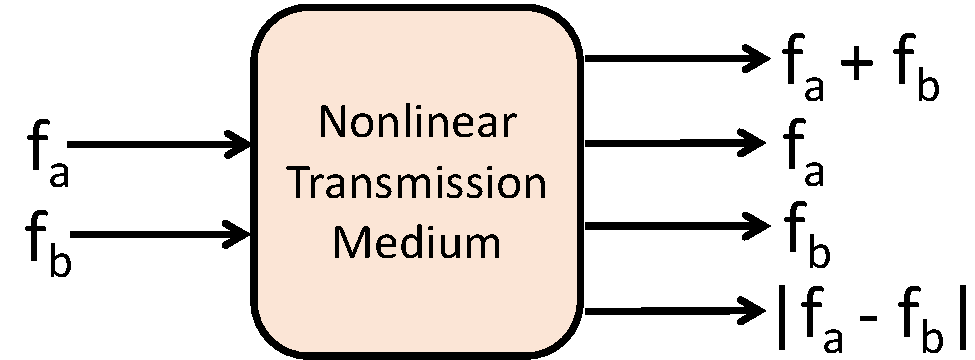
\includegraphics[width=.6\linewidth]{modulation}
	\caption{Self Demodulation of Sound Signals  When Transmitting Through the Human Body.}
	\label{fig:modulation}
\end{figure}

Researchers have found that sounds with different frequencies that transmitted through a nonlinear medium would interact with each other~\cite{pompei1998use}. This interaction produces new frequencies upon the combination of the sums and differences of the individual frequency components by Khokhlov-Zabolotskaya-Kuznetsov(KZK) parabolic nonlinear wave equation~\cite{novikov1987nonlinear}. 

Since the acoustic impedance of the human body is similar to that of water~\cite{kim2014sound}, the self-demodulation would occur in the human body as show in Fig.~\ref{fig:modulation}. 
The original sound signals with frequency $f_a$ and $f_b$ would introduce two more signals with frequency $f_a + f_b$ and $|f_a - f_b|$. For different person, the original signals generated have different frequency, so the low frequency signal $|f_a - f_b|$ are different, which can be utilized for user authetication.
%
Moreover, note that electronic devices has different acoustic property from that of human body. Therefore, those low frequent signals can be used for liveness detection.

%However, borrowing theories from \textit{compressed sensing}, the {\systemName} system can partially reconstruct the signal and obtain critical information such as the numbers appeared in a conversation, genders or even identities of the speakers, etc., from motion sensor readings, as discussed in Section~\ref{sec:threat}.

\subsection{Acoustic Attenuation}
Another effect helps {\shortname} to do spoof-proof authentication is the acoustic attenuation by human body.
%
It is known that human voice is emitted by the vocal organ and is a combination of mechanical vibrations with multiple  amplitudes and different  frequencies.
%
When a person speaks, the  airflow from the lungs through the trachea compresses the vocal cords causing vibrations to make sounds. The lung, trachea and vocal cord form a resonance chamber. 
%\begin{figure}[h]
%	\centering
%		\includegraphics[width=.4\linewidth]{background}
%	\caption{Background}
%	\label{fig:background}
%\end{figure}

Suppose the length of vocal cords is $d$, the lung volume is $V_0$ and the cross-sectional area at the vocal cords is $S$. According to the polytropic process equation, when the airflow moves $d$, the air pressure at the vocal cords can be expressed as follows,
\begin{displaymath}
P_1 = \frac{P_0 \cdot V^\gamma_0 }{(V_0 - d \cdot S)^\gamma},
\end{displaymath}
where $P_0$ is the normal atmospheric pressure, and $\gamma$ is a coefficient about the air specific heat. 
According to the definition of pressure, if the area at the vocal cords is $S_v$,  the force at the vocal cord is,
\begin{displaymath}
F_0 = P_1 \cdot S_v = \frac{S_v \cdot P_0 \cdot V^\gamma_0 }{(V_0 - d \cdot S)^\gamma}.
\end{displaymath}
When the force is applied to the vocal cords, vertical displacement occurs. 
According to the Newton’s second law of motion, we have,
\begin{displaymath}
F(t) = m a(t) + k x(t) + c v(t),
\end{displaymath}
where $F(t)$ is the external force, $v(t)$ is the speed, $x(t)$ is the vertical displacement, $c$ is the damping coefficient, and $k$ is the spring constant and m is the mass. 
The relation can further be explained as,
\begin{equation}
F(t) = m \frac{d^2 x(t)}{d t^2} + k x(t) + c \frac{x(t)}{d t}.
\label{eq:force}
\end{equation}

The vibration during an airflow pass the vocal cords can be separated into two phases. In the first phase, the airflow is passing the vocal cords which is considered to be a forced vibration with constant force $F_0$. After the airflow passed, in the second phase, the pressure of airflow disappears which leaves the system to vibrate on its own and this is called free vibration. In the forced vibration phase, after applying the Fourier transform to both side of e.q.~\eqref{eq:force}, we have,
\begin{displaymath}
\frac{F_0}{j \omega}(1-e^{-j\omega \delta t}) = - \omega^2 m X(\omega) + k X(\omega) + j \omega c X(\omega).
\end{displaymath}
That is,
\begin{displaymath}
X(\omega) = \frac{1-e^{-j\omega \delta t}}{-\frac{j m}{F_0} \omega^3 - \frac{c}{F_0} \omega^2 + \frac{j k}{F_0} \omega},
\end{displaymath}
where $X(\omega)$ is the spectrum of the vertical vibration signal and $\omega$ is the frequency. 
During the horizontal propagation of the vibration signal from the vocal cords to the throat, the vibration suffers from attenuation, and the corresponding model can be stated as follows,
\begin{displaymath}
x_s(t) = x(t) e^{-\alpha d},
\end{displaymath}
where $x_s(t)$ is the vertical displacement at the throat where the vibration has propagated, $x(t)$ is the vertical displacement at the vocal cords, $d$ is the propagation distance, and $\alpha$ is the attenuation coefficient. 
After applying the Fourier transform to both side of e.q.~\eqref{eq:force}, we have,
\begin{displaymath}
X_s(\omega) = X(\omega) e^{-\alpha d}.
\end{displaymath}
Note that $\alpha$ is related to the propagation medium. Wave propagation in body is dispersive by nature, which implies that different frequencies propagate with different attenuation coefficients at different velocities. Roughly speaking, the attenuation is small when the vibration signal propagates through the hard bone, whereas the attenuation is large through the soft tissue. Therefore, vibration waves generated at different positions at throat result in different values of $\alpha$ and $d$, which make the vibration signals unique at different positions. 
After putting all equations together, we obtain,
\begin{displaymath}
X_s(\omega) = \frac{(1-e^{-j\omega \delta t}) e^{-\alpha d}}{(-jm\omega^3 - c \omega^2 + jk\omega)(\frac{(V_0 - d \cdot S)^\gamma}{S_v \cdot P_0 \cdot V^\gamma_0 })}.
\end{displaymath}
For the same location of the human body, $m$, $c$ and $k$ are stable and belong to the same biometric feature. Each person’s lung volume and vocal cords are also different. Therefore, the vibration at the throat of different people can uniquely be identified, which can be leveraged for authentication. The propagation from electronic device to the target smartphone is different from vocal organ through human body. Thus, this effect is also valuable for liveness detection.


%\subsection{Voice Production}
%source-filter model, why our algorithm is user-independent. Similar source, different filter.
%\subsection{Voice Authentication System}
%Attacking (direct/indirect), here we only consider direct.

